\documentclass[a4paper,12pt]{report}

	
\usepackage[utf8x]{inputenc}
\usepackage[T2A]{fontenc}
\usepackage[english, russian]{babel}

% Опционно, требует  apt-get install scalable-cyrfonts.*
% и удаления одной строчки в cyrtimes.sty
% Сточку не удалять!
% \usepackage{cyrtimes}

% Картнки и tikz
\usepackage{graphicx}
\usepackage{tikz}
\usetikzlibrary{snakes,arrows,shapes}


% Увы, поля придётся уменьшить из-за листингов.
\topmargin -1cm
\oddsidemargin -0.5cm
\evensidemargin -0.5cm
\textwidth 17cm
\textheight 24cm

\sloppy



% Оглавление в PDF
\usepackage[
bookmarks=true,
colorlinks=true, linkcolor=black, anchorcolor=black, citecolor=black, menucolor=black,filecolor=black, urlcolor=black,
unicode=true
]{hyperref}

% Для исходного кода в тексте
% \newcommand{\Code}[1]{\texttt{#1}}

% Некоторая русификация.
% \usepackage{misccorr} % Oh shi^W^W, оно не работает с report.
\usepackage{indentfirst}
\renewcommand{\labelitemi}{\normalfont\bfseries{--}}

% На дворе XXI век, но пакет listings всё ещё не пашет с русскими комментариями!

% Пакет listings для простой вставки исходников
% \usepackage{listings}
% Параметры оформления
% \lstset{
% showspaces=false,
% showtabs=false,
% frame=single,
% tabsize=4,
% basicstyle=\ttfamily,
% identifierstyle=\ttfamily,
% commentstyle=\itshape,
% stringstyle=\ttfamily,
% keywordstyle=\ttfamily,
% breaklines=true
% }
% Русский в комментариях.
% \lstset{escapebegin=\begin{cyr},escapeend=\end{cyr}}



% А это взято из файла, сгенерённого doxygen
\usepackage{calc}
\usepackage{array}
\newenvironment{Code}
{\footnotesize}
{\normalsize}
\newcommand{\doxyref}[3]{\textbf{#1} (\textnormal{#2}\,\pageref{#3})}
\newenvironment{DocInclude}
{\footnotesize}
{\normalsize}
\newenvironment{VerbInclude}
{\footnotesize}
{\normalsize}
\newenvironment{Image}
{\begin{figure}[H]}
{\end{figure}}
\newenvironment{ImageNoCaption}{}{}
\newenvironment{CompactList}
{\begin{list}{}{
  \setlength{\leftmargin}{0.5cm}
  \setlength{\itemsep}{0pt}
  \setlength{\parsep}{0pt}
  \setlength{\topsep}{0pt}
  \renewcommand{\makelabel}{\hfill}}}
{\end{list}}
\newenvironment{CompactItemize}
{
  \begin{itemize}
  \setlength{\itemsep}{-3pt}
  \setlength{\parsep}{0pt}
  \setlength{\topsep}{0pt}
  \setlength{\partopsep}{0pt}
}
{\end{itemize}}
\newcommand{\PBS}[1]{\let\temp=\\#1\let\\=\temp}
\newlength{\tmplength}
\newenvironment{TabularC}[1]
{
\setlength{\tmplength}
     {\linewidth/(#1)-\tabcolsep*2-\arrayrulewidth*(#1+1)/(#1)}
      \par\begin{tabular*}{\linewidth}
             {*{#1}{|>{\PBS\raggedright\hspace{0pt}}p{\the\tmplength}}|}
}
{\end{tabular*}\par}
\newcommand{\entrylabel}[1]{
   {\parbox[b]{\labelwidth-4pt}{\makebox[0pt][l]{\textbf{#1}}\vspace{1.5\baselineskip}}}}
\newenvironment{Desc}
{\begin{list}{}
  {
    \settowidth{\labelwidth}{40pt}
    \setlength{\leftmargin}{\labelwidth}
    \setlength{\parsep}{0pt}
    \setlength{\itemsep}{-4pt}
    \renewcommand{\makelabel}{\entrylabel}
  }
}
{\end{list}}
\newenvironment{Indent}
  {\begin{list}{}{\setlength{\leftmargin}{0.5cm}}
      \item[]\ignorespaces}
  {\unskip\end{list}}


\begin{document}
	\begin{titlepage}
		\begin{center}
			\begin{LARGE}
				Отчет курсовой работе\\
					по курсу "Протоколы вычислительных сетей"\\
					по теме "Проектирование, реализация и тестирование почтового сервера SMTP"
			\end{LARGE}
		
			\begin{Large}
				\vspace{5cm}
				Студент: Спасенов И.В. ИУ7-41М\\
					Преподаватель: Оленев А. А. \\
				
				\vspace{10cm}2022 г.				   
			\end{Large}
			
		\end{center}
		 
	\end{titlepage}

\tableofcontents

\addcontentsline{toc}{chapter}{Введение}
\chapter*{Введение}


\subsection*{Задание. Вариант 10}

Используется вызов pselect и единственный рабочий поток. Журналирование в отдельном процессе. Нужно проверять обратную зону днс.

\subsection*{Цель и задачи}

Цель:
    Разработать \textbf{SMTP-сервер} с использованием одного потока и метода pselect(). Проверять обратную зону днс.

Задачи:
\begin{itemize}
    \item проанализировать \textbf{SMTP}-протокол и разработать конечный автомат обработки SMTP-сообщений;
    \item реализовать программу для получения и сохранения писем по протоколу \textbf{SMTP} на языке программирования \textbf{C};
    \item оформить расчетно-пояснительную записку.
\end{itemize}


\chapter{Аналитический раздел}

\section{SMTP}
SMTP (англ. Simple Mail Transfer Protocol — простой протокол передачи почты) — это широко используемый сетевой
протокол, предназначенный для передачи электронной почты в сетях TCP/IP.

SMTP впервые был описан в RFC 821 (\cite{rfc821}); последнее обновление в RFC 5321 (\cite{rfc5321}) включает масштабируемое
расширение — ESMTP (англ.  Extended SMTP). В настоящее время под «протоколом SMTP» как правило подразумевают
и его расширения. Протокол SMTP предназначен для передачи исходящей почты с использованием порта TCP 25.

\subsection{Реализуемые команды протокола SMTP}
\begin{enumerate}
	\item \textit{HELO} - открывает приглашение от клиента
    \item \textit{EHLO} - открывает приглашение от клиента
    \item \textit{MAIL FROM} - определяет отправителя сообщения
    \item \textit{RCPT TO} - определяет получателей сообщения
    \item \textit{DATA} - определяет начало сообщения
    \item \textit{RSET} - сбросить сеанс до состояния EHLO
    \item \textit{QUIT} - завершает сеанс SMTP
    \item \textit{NOOP} - не совершает операции

\end{enumerate}


\subsection{Метод мониторинга сетевых событий pselect}
Функция pselect как и select ждет изменения статуса нескольких файловых описателей.
Эти функции идентичны, за исключением 3-х отличий между ними:
\begin{enumerate}
\item Функция select использует время ожидания, которое задано в структуре struct timeval (с секундами и микросекундами), тогда как pselect использует struct timespec (с секундами и наносекундами).
\item Функция select может обновить параметр timeout, который показывает сколько времени прошло. Функция pselect не изменяет этот параметр.
\item Функция select не имеет параметра sigmask, и т.о. ведет себя также как функция pselect вызванная с этим параметром, установленным в NULL.
\end{enumerate}

В pselect отслеживаются 3 независимых набора описателей. Те, что перечислены в readfds, будут отслеживаться для того, чтобы обнаружить появление символов, доступных для чтения (говоря более точно, чтобы узнать, не будет ли блокировано чтение; описатель файла также будет указывать на конец файла); те описатели, которые указаны в writefds, будут отслеживаться для того, чтобы узнать, не заблокирован ли процесс записи; те же, что указаны в параметре exceptfds, будут отслеживаться для обнаружения исключительных ситуаций. При возврате из функции наборы описателей модифицируются, чтобы показать, какие дескрипторы фактически изменили свой статус.


\section{Сущности предметной области}
В результате проведенного исследования были выявлены следующие сущности предметной области: сервер, клиент, логгер, письмо.

\subsection{Сервер}

В полях данной сущности будет храниться информация необходимая для работы сервера.

\subsubsection{Спецификация}

\begin{enumerate}
	\item server\_fd - дескриптор сокета сервера
	\item clients\_list - список клиентов
	\item read\_fds - набор файловых дескрипторов, который служит для слежения за появлением данных, доступных для чтения из любого файлового дескриптора (для работы pselect)
	\item write\_fds - набор файловых дескрипторов, который служит для слежения за появлением места для записи данных в любой из файловых дескрипторов набора (для работы pselect)
	\item exceptions\_fds - набор файловых дескрипторов, который служит для слежения за появлением исключительных ситуаций на любом из файловых дескрипторов набора (для работы pselect)
	\item logger - логгер сервера
	\item maildir - путь к папке, в которой будут сохраняться письма
	\item max\_fd - максимальный номер дескриптора сокета (для работы pselect)
\end{enumerate}

\subsection{Клиент}

В полях данной сущности будет храниться информация необходимая для работы с клиентом. Для каждого пришедшего клиента создается такая сущность.

\subsubsection{Спецификация}

\begin{enumerate}
	\item smtp\_state - текущее состояние состояние клиента (состояние из конечного автомата)
	\item socket\_fd - дескриптор сокета клиента
	\item buffer\_input\_len - длина строки буфера принимаемых от клиента данных
	\item time - текущее время (нужно для работы таймера)
	\item buffer\_input - буфер принимаемых от клиента данных
	\item buffer\_output - буфер отправляемых  клиенту данных
	\item sent\_output\_flag - флаг отправки данных клиенту
	\item mail - письмо клиента
	\item next - указатель на следующего клиента
\end{enumerate}

\subsection{Письмо}

В полях данной сущности будет храниться информация о письме клиента.

\subsubsection{Спецификация}

\begin{enumerate}
	\item sender - отправитель письма
	\item recepients - получатели письма
	\item recepients\_num - количество получателей
	\item data - тело письма
	\item data\_capacity - длина тела письма
	
\end{enumerate}


\subsection{Логгер}

В полях данной сущности будет храниться информация для работы логгера.

\subsubsection{Спецификация}

\begin{enumerate}
	\item dir - директория, в которой будет храниться лог файл
	\item file - файл логгера
	\item msg\_queue\_key - ключ очереди сообщений логгера
	\item msg\_queue\_id - id очереди сообщений логгера
	
\end{enumerate}

\newpage


\subsection{ER-диаграмма предметной области}

Зависимость между сущностями предметной области может быть описана ER-диаграммой (~\ref{fig:er_diagram} ).

\begin{figure}
    \centering
    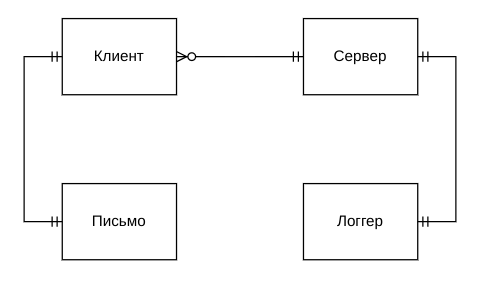
\includegraphics[width=\textwidth]{../images/er.png}
    \caption{ER-диаграмма предметной области}
    \label{fig:er_diagram}
\end{figure}

\newpage

\section{Достоинства и недостатки реализуемой архитектуры}

\subsection{Серверная часть SMTP агента}

Согласно условию задачи, в работе сервера предлагается использовать один поток выполнения и один отдельный поток
журналирования.

Достоинства варианта реализации:
\begin{itemize}
    \item простота реализации, отсутствует необходимость реализации разделяемой памяти и взаимодействия между процессами или потоками;
    \item отсутствие времени на переключение контекстов;
    \item благодаря неблокирующему вводу/выводу, сервер может обслуживать множество клиентов с достаточно высокой производительностью, при условии, что обработка занимает мало времени;
    \item логирование в отдельном процессе позволяет не блокироваться на операциях ввода/вывода при записи в файл или в терминал;
\end{itemize}

Недостатки данной архитектуры:
\begin{itemize}
    \item низкая производительность при длительной обработке клиентских команд;
    \item низкая отказоустойчивость (использование одного потока является менее надежным при возникновении фатальных ошибок в приложении, чем при наличии нескольих взаимозаменяемых потоков,);
    \item сложность масштабирования и использования всех аппаратных ресурсов системы.
\end{itemize}

Недостатки программной реализации с одним потоком выполнения и мультиплексированием можно уменьшить с  помощью
создания нескольких (пула) потоков с неблокирующим вводом/выводом и распределения нагрузки между ними.


\chapter{Конструкторский раздел}

\section{Конечный автомат состояний сервера}

На рис. ~\ref{fig:serverfsm} представлен сгенерированный с использованием \textit{fsm2dot} скрипта из \textit{autogen}
файла конфигурации конечного автомата \textit{server.def}.

\begin{figure}
    \centering
    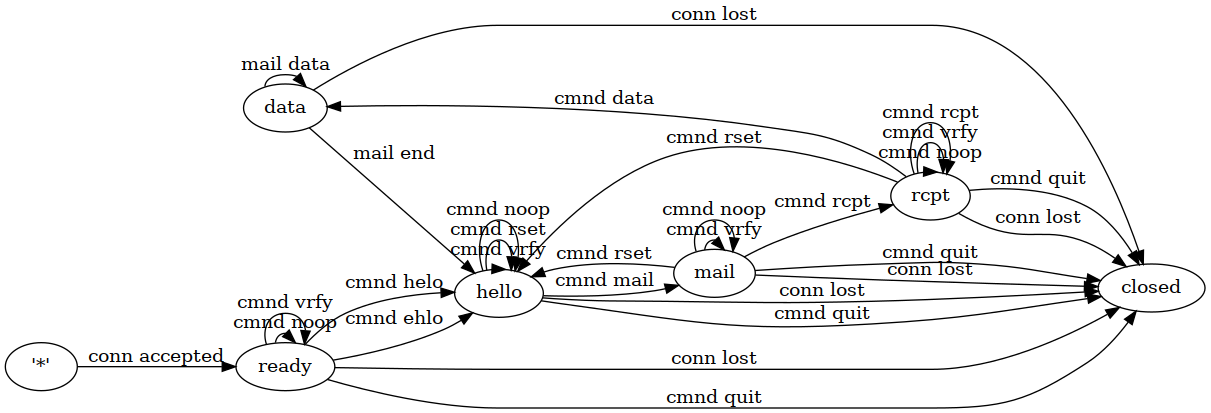
\includegraphics[width=\textwidth]{../images/serverfsm.png}
    \caption{Построенный граф конечного автомата SMTP сервера}
    \label{fig:serverfsm}
\end{figure}

\newpage


\section{Синтаксис команд протокола}
Ниже приведен формат команд сообщений протокола в виде регулярных выражений:

Регулярные выражения SMTP команд:
\begin{description}
    \item[NOOP]
    \texttt{\^{}NOOP}
    \item[HELO]
    \texttt{[Hh][Ee][Ll][Oo]\textbackslash{}\textbackslash{}s*(?<domain>.+)\textbackslash{}\textbackslash{}r\textbackslash{}\textbackslash{}n}
    \item[EHLO]
    \texttt{\^{}EHLO:}
    \item[MAIL]
    \texttt{\^{}MAIL FROM:}
    \item[RCPT]
    \texttt{[Rr][Cc][Pp][Tt] [Tt][Oo]:\textbackslash{}\textbackslash{}s*<(?<address>.+@.+)>\textbackslash{}\textbackslash{}r\textbackslash{}\textbackslash{}n}
    \item[VRFY]
    \texttt{\^{}VRFY:}
    \item[DATA]
    \texttt{\^{}DATA}
    \item[RSET]
    \texttt{[Rr][Ss][Ee][Tt]\textbackslash{}\textbackslash{}r\textbackslash{}\textbackslash{}n}
    \item[QUIT]
    \texttt{\^{}QUIT}
\end{description}

\section{Представление данных в системе}
На рис.~\ref{fig:uml_server_ph} и на рис.~\ref{fig:uml_server_log} представлены логическая и физическая
диаграммы представления данных в системе соответственно.


\begin{figure}
    \centering
    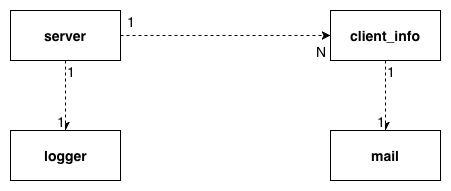
\includegraphics[width=\textwidth]{../images/uml_server_log.png}
    \caption{Логическая диаграмма представления данных в серверной части системы}
    \label{fig:uml_server_log}
\end{figure}

\begin{figure}
    \centering
    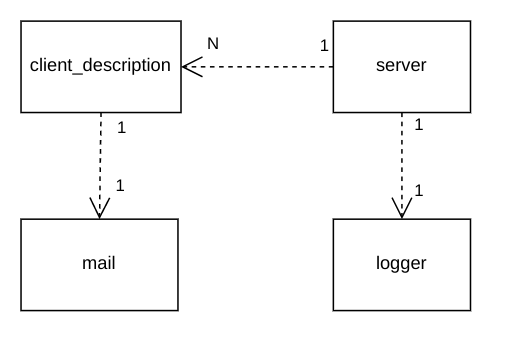
\includegraphics[width=\textwidth]{../images/uml_server_ph.png}
    \caption{Физическая диаграмма представления данных в серверной части системы}
    \label{fig:uml_server_ph}
\end{figure}



\newpage


\section{Обработка соединений в одном потоке выполнения}

Псевдокод обработки сервером клиентских соединений в одном потоке выполнения:

\begin{verbatim}
    Если пришло сообщение на сокет сервера 
        Обработать новое подключение и добавить нового клиента
    
    Цикл по всем дескрипторам сокетов клиента
    	    Если истек таймер ожидания команды от клиента
            Закрыть соединение с клиентом
        Если пришло сообщение на сокет клиента
            Обработать сообщение от клиента
        Если нужно отправить сообщение клиенту
            Отослать сообщение клиенту
        Если возникло исключение
            Закрыть соединение с клиентом

\end{verbatim}

\section{Обработка отправки в тексте письма символа окончания письма}
Если клиент в тексте письма добавит \textbackslash{}r\textbackslash{}n.\textbackslash{}r\textbackslash{}n то сервер закончит чтение, что будет ошибкой, поэтому в текщей реализации клиент заменяет все вхождения \texttt{\textbackslash{}r\textbackslash{}n.} в тексте письма клиента на \texttt{\textbackslash{}r\textbackslash{}n..}, сервер делает обратную замену.

\section{Осуществление журналирования}

Процесс журналирования запускается с помощью функции fork(), взаимодействие с процессом из родительского процесса осуществляется с помощью очереди сообщений.

\section{Хранение почты}

Для хранения почты, используется упрощенный формат Maildir. Maildir - формат хранения электронной почты, не требующий монопольного захвата файла для обеспечения целостности почтового ящика при чтении, добавлении или изменении сообщений. Каждое сообщение хранится в отдельном файле с уникальным именем, а каждая папка представляет собой каталог, имя которого совпадает с адресом получателя письма. 

Первоначально файл заполняется во временном месте (папка tmp), чтобы его невозможно было прочитать (из папки new) пока тот не будет полностью записан. Затем файл переносится в директорию new. 

Для того, чтобы имена файлов были уникальными, используется следующий формат: "(текущее значение секунд).(текущее значение миллисекунд).(случайное число)".



\chapter{Технологический раздел}

\section{Выбор языка и библиотек для разработки клиента}
В качестве языка реализации серверной части был выбран язык С стандарта с99. В качестве компилятора выбран gcc версии 9.3.0. Для выполнения IO мультиплексировании использовалась библиотека sys/select.h. Для автогенерации конечного автомата состояний сервера и структуры параметров для запуска сервера из командной строки использовался autogen.

\section{Выбор средств разработки}
В качестве среды разработки выступил Visual Studio Code 1.64.0

\subsection{Программное обеспечение, необходимое для сборки и запуска}
Для сборки и запуска сервера должны быть загружены следующие зависимости:

\begin{itemize} 
    \item gcc version 9.3.0
    \item GNU Make 4.2.1
    \item libconfig++-dev - требуется для libconfig.h;
    \item libedit-dev - требуется для arpa/nameser.h;
    \item autogen и autogen-libopts-devel
\end{itemize} 

\section{Сборка программы}

Сборка производится с помощью утилиты make(\cite{make}). make — утилита, автоматизирующая процесс преобразования файлов из одной формы в другую. Чаще всего это компиляция исходного кода в объектные файлы и последующая компоновка в исполняемые файлы или библиотеки.

Утилита использует специальные make-файлы, в которых указаны зависимости файлов друг от друга и правила для их удовлетворения. На основе информации о времени последнего изменения каждого файла make определяет и запускает необходимые программы.

Сборка SMTP сервера состоит из следующих целей:

\begin{enumerate}
	\item генерация исходных кодов конечного автомата и опций с помощью \textit{autogen};
    \item сборка сервера;
    \item сборка рпз, в котором помимо сборки pdf из tex файлов, осуществляется создание изображения графа конечного автомата состояний, графа cflow и графического описания make файлов;
    
\end{enumerate}



Полная сборка осуществляется с помощью следующей команды:
\begin{verbatim}
    make autogen_files && make server && make report
\end{verbatim}

Также в make файле присутствуют цели на запуск сервера, запуск сервера под valgrind и запуск тестов.

На рисунках \ref{ris:mkflow_first} 
и 
\ref{ris:mkflow_second} 
представлено графическое описание сборки программы.

\begin{figure}[h!]
\center{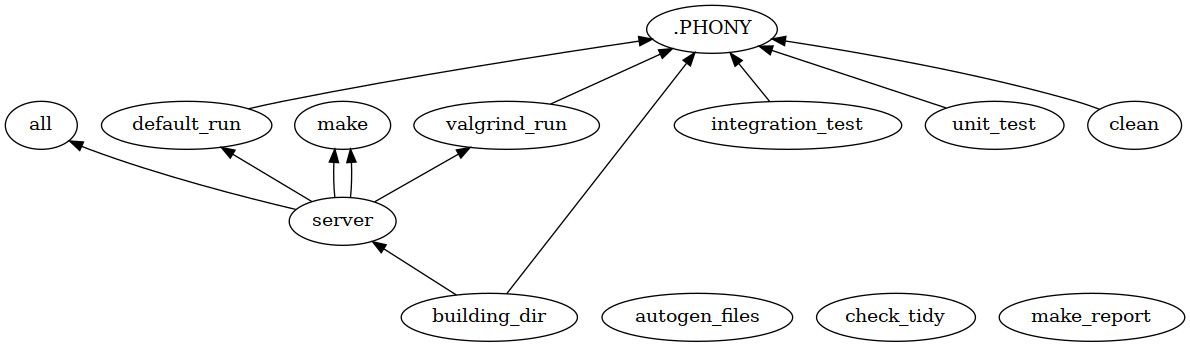
\includegraphics[width=1\linewidth]{../images/makefile_common.png}}
\caption{Графическое описание сборки программы часть 1}
\label{ris:mkflow_first}
\end{figure}

\begin{figure}[h!]
\center{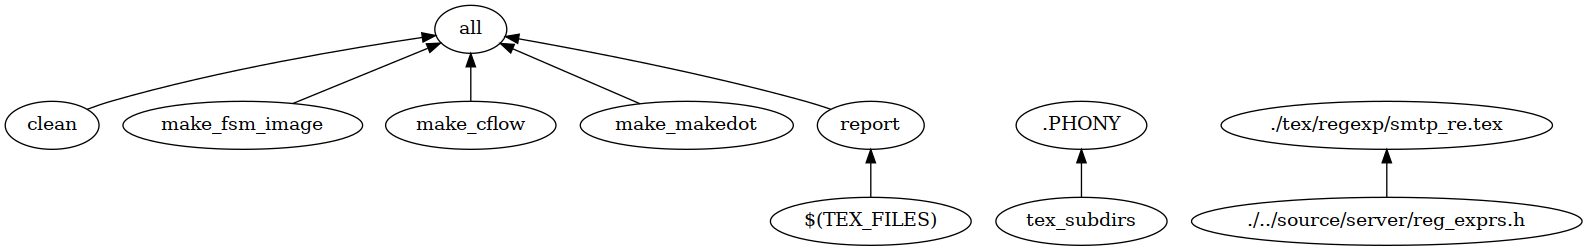
\includegraphics[width=1\linewidth]{../images/makefile_report.png}}
\caption{Графическое описание сборки программы часть 2}
\label{ris:mkflow_second}
\end{figure}

Запуск программы сервера содержит следующие параметры:
\begin{enumerate}
	\item -p - порт;
    \item -d - путь к директории с почтой;
    \item -l - Путь к директории с лог файлами;
\end{enumerate}



\subsection{Проверка обратной зоны dns}

Проверка осуществлется cледующим образом: сначала по номеру  дескриптора клиента с помощью функции getpeername заполняется структура sockaddr, затем из нее с помощью функции getnameinfo находится имя хоста, которое сравнивается с именем пришедшем в команде helo / ehlo.

\subsection{Граф вызова основных функций программы}

Для построения графа вызова была использована утилита cflow(\cite{cflow}). cflow - это генератор потоковых графиков, который является частью проекта GNU. Он считывает коллекцию исходных файлов C и генерирует потоковый график C внешних ссылок. Использует только исходные тексты и не нуждается в запуске программы.

На рисунке \ref{ris:calls} представлен граф вызова программы.

\begin{figure}[h!]
\center{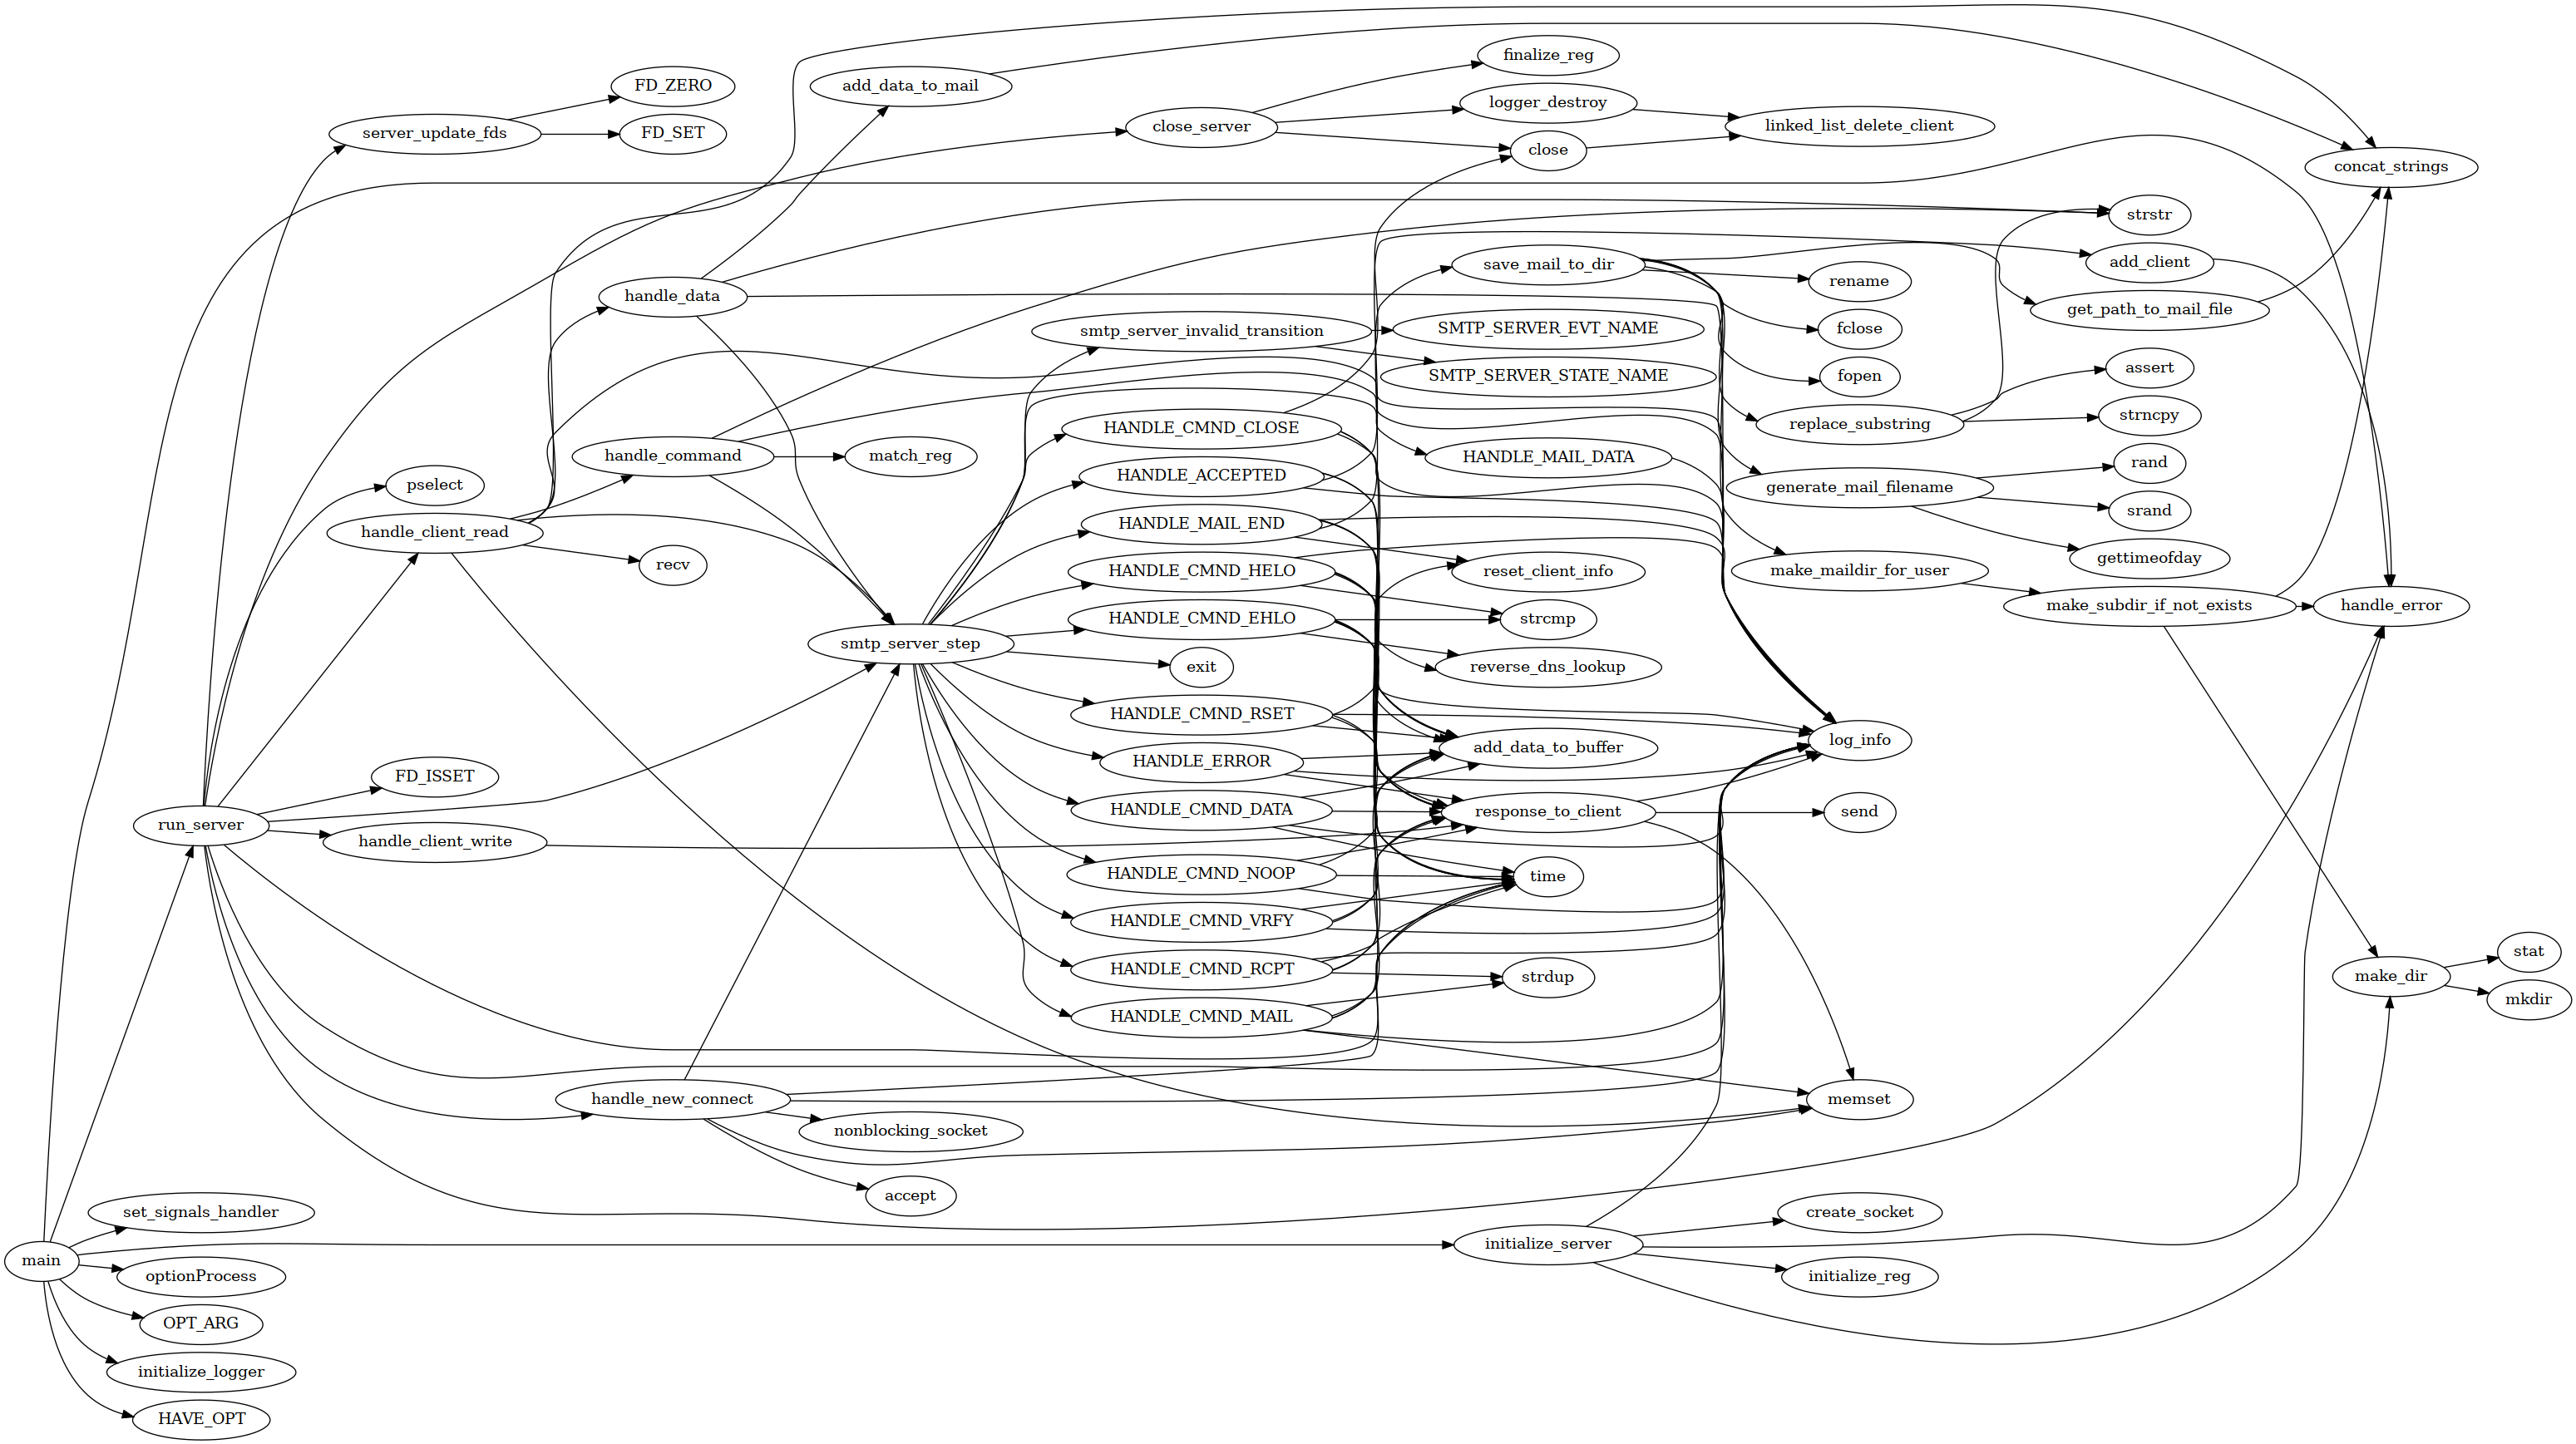
\includegraphics[width=1\linewidth]{../images/cflow.png}}
\caption{Граф вызовов основных функций программы}
\label{ris:calls}
\end{figure}

\newpage


\section{Тестирование}
Статический анализ кода проводился с помощью утилиты ctidy(\cite{ctidy}). clang-tidy - это инструмент “линтера” на C++ на основе clang. Его цель - предоставить расширяемую платформу для диагностики и исправления типичных ошибок программирования, таких как нарушения стиля, неправильное использование интерфейса или ошибки, которые могут быть выявлены с помощью статического анализа. clang-tidy является модульным и предоставляет удобный интерфейс для написания новых проверок.

\subsubsection{Модульное тестирование}
 
 Модульное тестирование проводилось с помощью библиотеки check.h \cite{check}. Check - это платформа модульного тестирования для C. Он имеет простой интерфейс для определения модульных тестов. Тесты выполняются в отдельном адресном пространстве, способен обнаруживать ошибки кода, которые приводят к сбою сегментации или другим проблемам. 
 
 Результаты тестирования предствлены ниже.
\begin{verbatim}
    100%: Checks: 11, Failures: 0, Errors: 0
\end{verbatim}
 
\subsubsection{Интеграционное тестирование}

Проводилось интеграционное тестирование сервера по следующим пунктам:
\begin{enumerate}
	\item передача одному получателю маленького сообщения;
	\item передача нескольким получателям маленького сообщения;
	\item передача одному получателю маленького сообщения с пустым адресом отправителя;
    \item передача одному получателю большого сообщения;
    \item передача одному получателю несколько сообщений подряд;
    \item передача неавалидных команд;
    \item передача rset после команд mail и rcpt;
    \item передача quit после команд helo, mail, rcpt;
    \item передача в тексте сообщения \texttt{\textbackslash{}r\textbackslash{}n..} и замену его на \texttt{\textbackslash{}r\textbackslash{}n.};
\end{enumerate}

Тестирование проводилось с помощью скрипта, написанного на языке Python в файле test.py, для соединения с сервером использовалась библиотека socket.

Результат тестирования:
\begin{verbatim}
PASS test 1
PASS test 2
PASS test 3
PASS test 4
PASS test 5
PASS test 6
PASS test 7
PASS test 8
PASS test 9
\end{verbatim}


Для поиска утечек использовась утилита valgrind(\cite{valgrind}). Valgrind — инструментальное программное обеспечение, предназначенное для отладки использования памяти, обнаружения утечек памяти, а также профилирования. 

Valgrind по сути является виртуальной машиной, использующей методы JIT-компиляции, среди которых — динамическая перекомпиляция. То есть, оригинальная программа не выполняется непосредственно на основном процессоре. Вместо этого Valgrind сначала транслирует программу во временную, более простую форму, называемую промежуточным представлением (Intermediate Representation, сокр. IR), которая сама по себе не зависит от процессора и находится в SSA-виде. После преобразования инструмент может выполнять любое необходимое преобразование IR до того, как Valgrind оттранслирует IR обратно в машинный код и позволит основному процессору его исполнить. Её используют, даже несмотря на то, что для этого может использоваться динамическая трансляция (то есть, когда основной и целевой процессоры принадлежат к разным архитектурам). Valgrind перекомпилирует двоичный код для запуска на основном и целевом (или его симуляторе) процессорах одинаковой архитектуры.

При проведении тестирования valgrind был запущен с настройками, представленными ниже
\begin{verbatim}
    --tool=memcheck --track-origins=yes  --leak-check=full --show-reachable=yes
\end{verbatim}

Отчет valgrind после прогона тестов:
\begin{verbatim}
==166488== 
==166488== HEAP SUMMARY:
==166488==     in use at exit: 0 bytes in 0 blocks
==166488==   total heap usage: 34 allocs, 34 frees, 536,445 bytes allocated
==166488== 
==166488== All heap blocks were freed -- no leaks are possible
==166488== 
==166488== For lists of detected and suppressed errors, rerun with: -s
==166488== ERROR SUMMARY: 0 errors from 0 contexts (suppressed: 0 from 0)
==166487== 
==166487== HEAP SUMMARY:
==166487==     in use at exit: 0 bytes in 0 blocks
==166487==   total heap usage: 25,774 allocs, 25,774 frees, 13,498,089 bytes allocated
==166487== 
==166487== All heap blocks were freed -- no leaks are possible
==166487== 
==166487== For lists of detected and suppressed errors, rerun with: -s
==166487== ERROR SUMMARY: 298 errors from 1 contexts (suppressed: 0 from 0)
\end{verbatim}




\addcontentsline{toc}{chapter}{Выводы}

\chapter*{Выводы}


В результате выполнения курсового проекта была достугнута поставленная цель, а именно разработан
\textbf{SMTP-сервер} с использованием одного потока и метода pselect(), осуществляющее прием и сохранение писем
для дальнейшей поставки их пользователям, с проверкой обратной зоны dns.

Во время выполнения работы были выполнены следующие задачи:
\begin{itemize}
    \item проанализирован \textbf{SMTP}-протокол и разработан конечный автомат обработки SMTP-сообщений;
    \item реализована программу для получения и сохранения писем по протоколу \textbf{SMTP} на языке программирования \textbf{C};
    \item оформлена расчетно-пояснительную записка;
	\item написаны модульные и интеграционные тесты.
\end{itemize}



  \newpage
 \addcontentsline{toc}{section}{Список литературы}
    \begin{thebibliography}{11} 
    
    \bibitem{rfc821} Протокол передачи данных SMTP в редакции RFC821 https://www.ietf.org/rfc/rfc821.txt
    
    \bibitem{rfc5321} Протокол передачи данных SMTP в редакции RFC5321 https://www.ietf.org/rfc/rfc5321.txt
    
      \bibitem{rfc2045} Формат SMTP сообщений в редакции RFC2045 https://www.ietf.org/rfc/rfc2045.txt
    
    \bibitem{io_multi} Обзор методов IO мультиплексирования https://habr.com/ru/company/infopulse/blog/415259/
    
    \bibitem{poll_info} Устройство системного вызова poll https://programming.vip/docs/i-o-multiplexing-poll-system-call.html
    
     \bibitem{time_c99} C99 standard (ISO/IEC 9899:1999): 7.23.2.4 The time function (p: 341) 
     \\http://www.open-std.org/jtc1/sc22/wg14/www/docs/n1124.pdf
     
     \bibitem{c11} C11 standard (ISO/IEC 9899:201x): http://www.open-std.org/jtc1/sc22/wg14/www/docs/n1570.pdf
     
      \bibitem{mx_info} представлено MX записи https://semantica.in/blog/chto-takoe-mx-zapis-domena.html
      
     \bibitem{make} официальный сайт разработчиков make   https://www.gnu.org/software/make/manual/make.html
    
     \bibitem{valgrind} официальный сайт разработчиков valgrind https://valgrind.org/
    
     \bibitem{cflow} официальный сайт разработчиков cflow  https://www.gnu.org/software/cflow/manual/cflow.html
     
      \bibitem{ctidy} официальный сайт разработчиков clang tidy   https://clang.llvm.org/extra/clang-tidy/
    \bibitem{check} официальный сайт разработчиков check  https://libcheck.github.io/check/
    \end{thebibliography}


\end{document}

